\documentclass[Main]{subfiles}
\begin{document}

\chapter{Mathematical Preliminaries}
%%%	Intro	%%%
%\_-_-_-_-_-_-_-_-_-_-_-_-_-_-_-_-_-_-_-_-_-_-_-_-_-_-_-_-_-_-_-_-_-_-_-_-_-_-_-_-_-_-_-_-_-_-_-_-_-_-_-_-_-_-_%
	The interaction between mathematics and Quantum Field Theory are complex and highly not trivial.
	Since contemporary quantum field theory is mainly developed as a quantization of classical fields, the mathematical foundation of classical field theory represents a necessary step towards the understanding of the foundations of field theory.
	
	%Goal of this section is to introduce the three  building blocks of classical field theory, namely \emph{vector bundles}, \emph{globally hyperbolic spacestimes} and \emph{Green hyperbolic operators}.
	Goal of this section is to introduce the three  building blocks of \emph{"pre-quantum" field theory} , by this we mean the theory that describes the classical analogue of quantum theory that, in turn, describes the elementary particles.
	Namely these are the \emph{vector bundles}, \emph{globally hyperbolic spacestimes} and \emph{Green hyperbolic operators}.
	Given the purpose of this thesis, we shall not dwell on the structures typical of the quantum framework (such *-algebras).
	We assume that the reader is familiar with the basic notions of differential geometry, external calculus and, to a minor extent, of general relativity.
%\_-_-_-_-_-_-_-_-_-_-_-_-_-_-_-_-_-_-_-_-_-_-_-_-_-_-_-_-_-_-_-_-_-_-_-_-_-_-_-_-_-_-_-_-_-_-_-_-_-_-_-_-_-_-_%
%\_-_-_-_-_-_-_-_-_-_-_-_-_-_-_-_-_-_-_-_-_-_-_-_-_-_-_-_-_-_-_-_-_-_-_-_-_-_-_-_-_-_-_-_-_-_-_-_-_-_-_-_-_-_-_%
	\section{Fiber Bundles}
		\emph{Fiber bundles} are the stage for the kinematics of classical and quantum fields.
		Its main role is to encode the kinematic configurations of an arbitrary field theory through the concept of
		\emph{sections}.
		
		\subsection{Formal Definition}
			Although it would be possible to present the concept of \emph{bundle} in a more general way through the language of categories, for the sake of this work it will be sufficient to consider only the case of \emph{smooth bundles}.
			\begin{definition}[Fiber Bundle]\label{Def:SmoothBundle}
				We call a \emph{Smooth (Fiber) Bundle}  a quadruple $(E,M,Q,\pi)$ where:
				\begin{itemize}
					\item[-] $E,M,Q$ :  smooth manifolds called respectively \emph{Total Space}, \emph{Base Space}, \emph{Typical Fiber}.
					\item[-] $\pi : E \rightarrow M $ smooth function (called \emph{Bundle Projection})
				\end{itemize}
				Endowed with a \emph{Local Trivialization}:
				\begin{itemize}
					\item $\forall x \in M \; \exists$ a couple $(U, \chi)$ (called \emph{local trivialization})
					\begin{itemize}
						\item $U$ : neighbourhood of $x$
						\item $\chi$ :$\pi^{-1}(U) \rightarrow U \times Q$ : diffeomorphism
							%DaRivedere
 							\footnote{surjectivity $\Rightarrow$ $\pi^{-1}(U) \neq \emptyset$.} 
 							\footnote{cartesian product of topological space is a topological space with the direct product topology.}
					\end{itemize}
					such that the natural projection $p_1 : U \times F \rightarrow U$ satisfies the following equation: $$p_1 \cdot \chi = \pi \vert_{\pi^{-1}(p)}$$

					\textit{i.e.}: the following graph commutes:
					
					\begin{center}
					\begin{tikzpicture}
						 \matrix (m) [matrix of math nodes,row sep=3em,column sep=4em,minimum width=2em] {
     						\pi^{-1}(U) & U \times Q \\
     						U &  \\};
 						 \path[-stealth]
 							(m-1-1) edge node [left] {$\pi$} (m-2-1)
            				edge [right] node [above] {$\chi$} (m-1-2)
    						(m-1-2) edge [right] node [below] {$p_{1}$} (m-2-1);;
					\end{tikzpicture}					
					\end{center}


				\end{itemize}
			\end{definition}

			\begin{figure}[h!]
  				\caption{The complete fiber bundle Structure.}
  				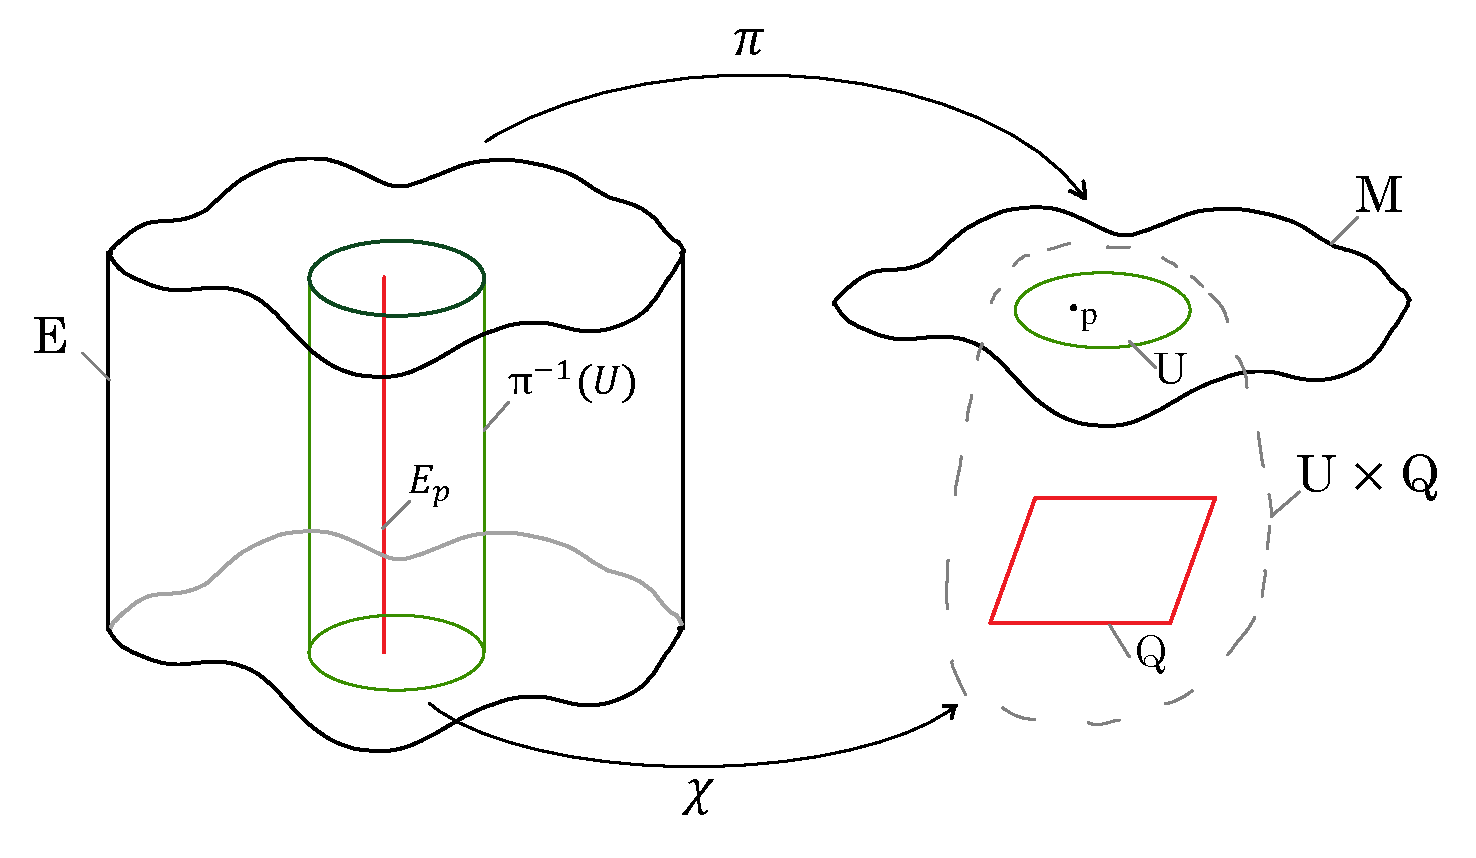
\includegraphics[width=0.5\textwidth]{Pictures/fiberbundle}				
%  				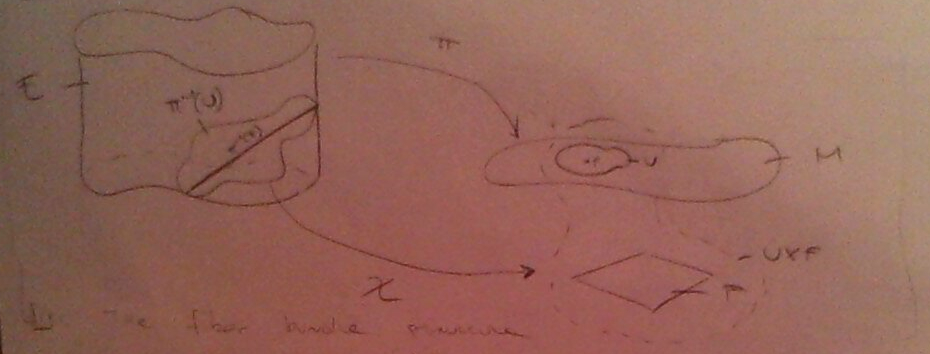
\includegraphics[width=0.5\textwidth]{Pictures/FiberBundle}
  				\centering
			\end{figure}
%			\begin{notationfix}
				It is customary to refer to a vector bundle specifying only its total space:
				\begin{displaymath}
					\gls{Bundle}%E= ( E,\pi, B ; F)
				\end{displaymath}
			 	In the following we adopt this convention whenever this does not lead to misunderstandings.
%			\end{notationfix}
			
			\vspace{2mm}
%			\begin{observation}
				For all $p\in M$ we refer to the submanifold $E_{p} := \pi_{-1}(p) \subset E $ as \emph{fiber over the point p}.
				\\
				Every fiber $E_p$ is diffeomorphic to the typical fiber $F$ through the local trivialization charts.
%			\end{observation}		

			\vspace{2mm}
%			\begin{notationfix}
				Since  Definition \ref{Def:SmoothBundle}  prescribes the existence of local trivializations only,
				we say that a smooth bundle E is \emph{(globally) trivial} if $E \simeq M \times Q$ i.e there exists a trivialization of $E$ which is defined everywhere.
%				\\
%				Note that Definition \ref{Def:SmoothBundle}  prescribes the existence of local trivializations only.
%			\end{notationfix}
			\vspace{3mm}
			
			When a smooth fiber bundle $(E,\pi,M;Q)$ is considered, in addition to the typical functions of the bundle $(\pi, \chi_{\alpha})$ also the local charts $(U_{\alpha_k}, \phi_{\alpha_k})_{k = E,M,Q}$, provided by the atlases of E, M and Q, should be provided.
			%should be taken in account also  the local charts $(U_{\alpha_k}, \phi_{\alpha_k})_{k = E,M,Q}$ provided by the atlases of $E,M$ and $Q$:
			\begin{definition}[Bundle atlas]
				We calla a \emph{Bundle Atlas} a collection of local charts which trivializes $E$. I.e. triples  $(U_\alpha, \psi_\alpha, \chi_\alpha)$ where:
				\begin{itemize}
					\item $U_\alpha$ is a open set in $M$ such that $\bigcup_{\alpha} U_{\alpha} \supseteq M$.
					\item $\chi_\alpha$  is a local trivialization.
					\item $(U_\alpha,\psi_\alpha)$ is a local chart on $M$.
				\end{itemize}		
			\end{definition}
%			\begin{observation}

			Notice that when are given a local chart $(U_\alpha, \psi_\alpha^{(M)} )$ on M and a local chart $(U_\alpha^{(Q)}, \psi_\alpha^{(Q)})$ on the fiber manifold it is possible to construct a chart on the total space:	
				\begin{displaymath}
							\psi^{(E)}_\alpha = \psi_\alpha^{(M)} \times  \psi_\alpha^{(Q)} \circ \chi_\alpha
				\end{displaymath}	
%			\end{observation}
			\vspace{3mm}			
			
			Endowing the bundle manifolds with other additional structures, we can introduce important subclasses of smooth bundles:
			\begin{definition}[Vector Bundle]
				We call \emph{Vector Bundle} a smooth bundle $E=(E,\pi,M;V)$ such that:
				\begin{itemize}
					\item The typical fiber $V$ is a finite dimensional vector space.	
					\item All trivializations $\chi_{\alpha} $ are diffeomorphisms such that:
						\begin{displaymath}
							\chi_{\alpha}\vert_{\pi^{-1}(p)} \in \mathbb{GL}(n, \mathbb{R})
						\end{displaymath}
				\end{itemize}
			\end{definition}

		\subsection{Cross Sections}
			Sections represent the natural mathematical object to encode a $Q-$ valued classical field over the space $M$:			
%			\begin{definition}[Smooth Section]
%				We call \emph{Smooth Section} a function $\phi : M \rightarrow E$ such that:
%					\begin{itemize}
%						\item $\phi$ smooth.
%						\item $\pi \cdot \phi = \IdMap_M$ 
%					\end{itemize}
%			\end{definition}
			\begin{definition}[Smooth Section]
				We call \emph{Smooth Section} 	any $\phi\in C^\infty(M;E)$ such that $$\pi\circ\phi = id|_M$$		
			\end{definition}
%			\begin{notationfix}
				We refer to:
					\begin{itemize}
						\item \emph{Global section} $\Leftrightarrow$ $\textrm{dom}(\phi) = M$
						\item \emph{Local section} $\Leftrightarrow$ $\textrm{dom}(\phi) \subset M$
					\end{itemize}
				We denote the set of all global smooth sections of the bundle $E$  as:
				\begin{displaymath}
					\gls{Sections}
				\end{displaymath}
%			\end{notationfix}
\ifToninus
		\begin{observation}
			In general, \gls{Sections} is an infinite dimensional manifold. 
			\\
				In case of vector bundles it is also a linear Frechet space\cite{Kriegl}.
			\\
			In the rather particular case of the tangent bundle on a smooth manifolds the sections are also called "vector fields" and indicated as:
			\begin{displaymath}
				\mathfrak{X}(M) = \Gamma^\infty(TM)
			\end{displaymath}
		\end{observation}
\else
			generally this space is an infinite dimensional manifold.
			In case of vector bundles it is also a linear Frechet space\cite{Kriegl}.
\fi

			
			
		\subsection{Mapping between Bundles}
			%Bundle morphism
			Consider two smooth bundles $E=(E,\pi,M; Q)$ and $E'=(E',\pi',M; Q')$ on the same base space $M$.
			\begin{definition}[Bundle map (\emph{Fiber Preserving map})]\label{Def:BundleMap}
				We call \emph{bundle map} a smooth function $\phi: E \rightarrow E'$ such that:			
			 	\begin{displaymath}
			 		\phi(E_{x})= F_{x} \qquad \forall x \in M.
			 	\end{displaymath}
				i.e.:
				
				\centering
				\begin{tikzpicture}
					 \matrix (m) [matrix of math nodes,row sep=3em,column sep=4em,minimum width=2em] {
						E & & F \\
       					& M & \\};
					\path[-stealth]
    					(m-1-1) edge node [left] {$\pi_{E}$} (m-2-2)
   		         		edge [right] node [above] {$\phi$} (m-1-3)
    					(m-1-3) edge node [right] {$\pi_{F}$} (m-2-2);
				\end{tikzpicture}
			\end{definition}
%			\begin{observation}
				Definition \ref{Def:BundleMap} is a special case of \emph{bundle-morphism}. (see for example \cite{G.Sardanashvily2013})
%			\end{observation}

			%pullback bundle
			Consider a smooth manifold $N$, a (smooth) fiber bundle $E=(E,\pi,M;Q)$, and a smooth function $f: N \rightarrow M$. it is possible to induce\cite{Husemoller} a bundle structure from $M$ to $N$:
			\begin{definition}[Pull-Back Bundle]
				We call \emph{pull-back bundle} of E a triple $f^* (E) = (f^* (E) , \pi^*,N)$ such that:
				\begin{itemize}
					\item $f^* (E) =  \big\{ (b',e) \in N \times E \quad \big\vert \; f(b') = \pi(e) \big\} $
					\item $\pi^*:f^* (E) \rightarrow N $ such that $ \pi^* (b',e) = \textrm{pr}_1 (b',e)= b' $
				\end{itemize}
				where $p_1 : U \times F \rightarrow U$ is the natural projection  on the first entry.
			\end{definition}
			\begin{proposition}
				$f^* (E) = (f^* (E) =, \pi^*,N)$ is a smooth bundle with typical fiber $Q$.
			\end{proposition}
			\begin{proof}
				To complete the fiber bundle structure it is sufficient to provide a local trivialization atlas.
				\\
				$\forall ( U, \phi)$ local trivialization on $(E, \pi, M)$  consider $\psi: f^* E \rightarrow N \times Q$ such that $\psi( b',e) = \bigg( b', pr_2 \big( \phi(e)\big)\bigg)$.
				\\
				Then $(f^{-1}(U),\psi)$ is a local trivialization of the pull-back bundle and the fiber of $f^*E$ over a point $b'\in B'$  is just the fiber of E over $f(b')$.
			\end{proof}

			
			%mor bundle
			It is also noteworthy that, given any two vector bundles $E =(E,\pi,M,Q)$ and $E =(E',\pi',M',Q')$, we can construct 	naturally a third fiber bundle.\\
			Consider $\Hom(E,E')$ the set of all the fiber preserving map between the two bundles:
			\begin{definition}[Bundle of homomorphisms]
				We call \emph{bundle of homomorphisms} a fiber bundle $\Hom(E,E')$ over the base space $M$ such that the fiber over a base point $p\in M$ is the infinite dimensional manifold $\Hom(E_p,E'_p)$ isomorphic to $\Hom(Q,Q')$.
			\end{definition}
%			\begin{notationfix}
				We shall write $End(E)$ for $\Hom(E,E)$ and we call it bundle of endomorphism, whose typical fiber is $\textrm{End}(Q)$.
%			\end{notationfix}
			\begin{remark}
				If $F,F'$ are vector bundle then the fiber of  $\Hom(F,F')$ over a base point $p\in M$ is $\Hom(F_p,F'_p)$, which is a vector space isomorphic to the vector space $\Hom(V,V')$ of linear applications from $V$ to $V'$
			\end{remark}
	
		\subsection{Tangent Bundles}
			The \emph{tangent} bundle is a natural structure defined on any smooth manifold, it represents the canonical example of  non-trivial vector bundle.
						
			\begin{definition}[Tangent Bundle]
				We call \emph{tangent bundle of M} the smooth vector bundle $TM=(TM,\tau,M;\Real^m)$ such that:
				\begin{itemize}
					\item The total space is the union of all tangent spaces to 
						$$TM \coloneqq \underset{p \in M}{\sqcup} T_pM  \equiv \bigcup_{x\in M} {x}\times T_x M$$
					\item The bundle projection maps each tangent vector $v\in  T_pM$ to the correspondent base point  $p$;
						$$\tau : (p,v_p) \mapsto p $$
				\end{itemize}
			\end{definition}			
			In a similar fashion it is possible to construct a structure dual to $TM$:
			\begin{definition}[Cotangent Bundle]
				We call \emph{cotangent bundle} the vector bundle $T^*M$ builded by disjoint union of the dual tangent space $T_p^*M $.
			\end{definition}
			Furthermore, this construction can be repeated for any tensor product of the tangent and cotangent spaces, \textit{i.e.}:
				\begin{itemize}
%					\item \emph{Cotangent Bundle} $T^*M$ is build by 
					\item The \emph{Tensor Bundle} $T^{(k,l)}M$ is build by disjoint unions of the tensor product of tangent space with itself:
					\begin{displaymath}
						T^{(k,l)}_ p M = \underbrace{T^*_pM \otimes \cdots \otimes T^*_pM}_{\textrm{k-times}} \otimes
						\underbrace{T_pM \otimes \cdots \otimes T_pM}_{\textrm{l-times}}
					\end{displaymath}
					\item The \emph{k-form Bundle} $ \bigwedge^m( T^*M)$ is build by disjoint unions of the antisimmetrized tensor product of the dual tangent space with itself.
				\end{itemize}
%			\end{observation}
			
			
			\subsubsection{Tautological one-form and symplectic form.}
					\begin{remark}
%					\begin{notationfix}
						In the context of Classical mechanics is customary to refer to the cotangent bundle $T^*Q$ over the smooth manifold  $Q $ - called \emph{Configuration Space}  - as \emph{Phase Space}.
%					\end{notationfix}
					\end{remark}

					Since $TQ$ and $T^*Q$ are diffeomorphic , it might seem that there is no particular reason in treating these two spaces separately, but this is not the case.
					There are certain geometrical objects that live naturally on $T^*Q$ , not on $TQ$.
					Of greatest interest % in mathematical-physics 
					are the Poincaré forms\cite{Frankel2003}.
	
					Consider a smooth manifold $Q$ and call $\Phase=T^*Q$ the corresponding cotangent bundle.
					\begin{definition}[Tautological (Poincaré) 1-form]
						We call \emph{tautological form} the 1-form over $\Phase$:
						\begin{displaymath}
							\theta_0 \in \Gamma^\infty (T^*\Phase)
						\end{displaymath}
					such that the action on a generic point $ \omega_{\alpha_p} \in T_{\alpha_p}M$ ( in the fiber of $\alpha_p$, which in turn is a one-form on the fiber of $p\in Q$) is given by:
						\begin{displaymath}
						\theta_0 \big(\alpha_p \big): T_{\alpha_p}\Phase \rightarrow \Real \qquad : \; \omega_{\alpha_p} \mapsto \alpha_q \circ T \tau^*_Q \big( \omega_{\alpha_p} \big)
						\end{displaymath}
					where $T$ is the \emph{tangent map}, namely the bundle-morphism which act on each fiber as the differential map $d (\tau^*_Q)$.
					\end{definition}
					\begin{figure}[h!]
						\centering
   						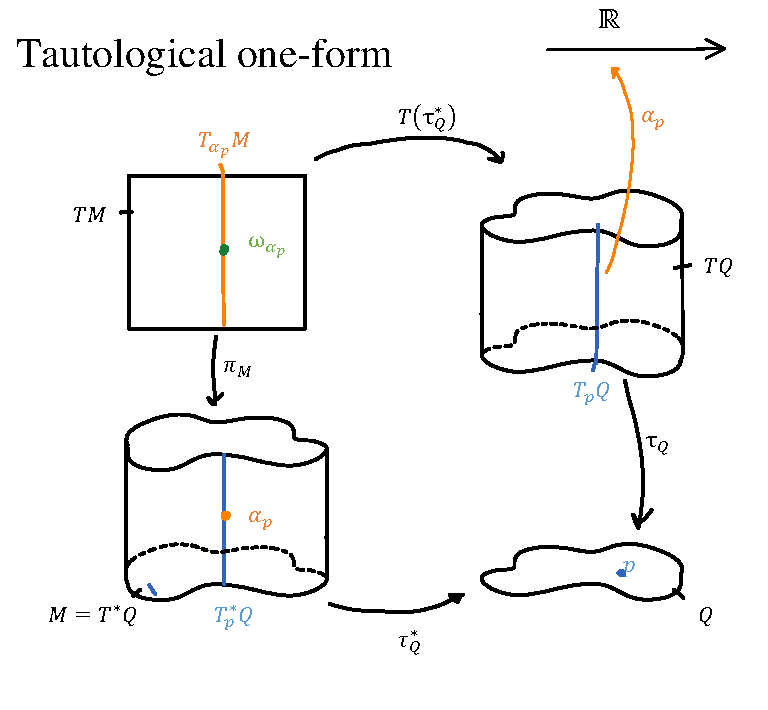
\includegraphics[width=0.5\textwidth]{Pictures/Tautological1Form} 
 						\caption{The definition of tautological 1-form is achieved exploiting the concept of \emph{Tangent map} and remembering that $\alpha_p: T_p \Phase \rightarrow \Phase$ is a linear functional.} 
  						\centering
					\end{figure}	
%					\begin{remark}	
%					\begin{notationfix}
						In the context of classical mechanics we define a  special set of coordinates on the cotangent bundle of a manifold called \emph{canonical coordinates}.
						They are usually written as a set of $(q^i,p_j)$ where ${q_i}$ are denoting the coordinates on the underlying manifold and the ${p_j}$ are denoting the conjugate momenta, which are decompositions of 1-forms in $T_p^*M$ on the dual natural basis $d q^J$ in the cotangent bundle at the point $q$ in the manifold.
%					\end{notationfix}
%					\end{remark}
	
%					\begin{observation}
						In canonical coordinates the tautological one-form assumes the famous expression:
						\begin{displaymath}
							\theta_0 = \sum_{i=1}^n {p_i} d q^i
						\end{displaymath}
						(note that $d q^i$ is a 1-form on $T^*M$ calculated with respect to the coordinate on the bundle. One should not confuse it with the 1-natural form $d q^i \in T^*_p M$.)
%					\end{observation}

	
%					The claim is proved by the following definition:
					This allows us to define a natural symplectic structure on any phase space:
					\begin{definition}[Canonical (Poincarè)  symplectic form]\label{Def:NatSymForm}
						We call \emph{Canonical (Poincarè)} form the symplectic:
						\begin{displaymath}
							\omega_0 \coloneqq -d \theta_0
						\end{displaymath}
						In canonical coordinates it assumes the renown expression:
						\begin{displaymath}
							\omega_0 \coloneqq \sum_{i=1}^n  d q^i \wedge d p_i
						\end{displaymath}
					\end{definition}
					
		\subsection{Jet Bundles}\label{Sect:JetBundles}
			The jet bundle is a %certain 
			construction that makes a new smooth fiber bundle out of a given bundle. The first step is to identify the typical fiber for this construction.

			Suppose $M$ is an m-dimensional manifold and that $(E, \pi, M)$ is a fiber bundle. 
			Consider the set of all the local sections whose domain contains $p$:
			\begin{displaymath}
				\Gamma^\infty (p) \coloneqq \big\{ \sigma \in \Gamma^\infty(E) \quad \big\vert\:  p \in \dom(\sigma)  \big\}
			\end{displaymath}

			We define an equivalence relation between such section \emph{up to r-th order}:
			\begin{definition}[r-jet equivalence]
				Two sections $\sigma, \eta \in \Gamma^\infty(p)$ have the \underline{same \emph{r-jet} at $p$} $(\sigma \sim \eta)$ iff:
				\begin{displaymath}
					\left.\frac{\partial^{|I|} \sigma^{\alpha}}{\partial x^{I}}\right|_{p} = \left.\frac{\partial^{|I|} \eta^{\alpha}}{\partial x^{I}}\right|_{p} \quad \forall I\in \Natural^m_0 \, \vert \, 0 \leq |I| \leq r.
				\end{displaymath}	
				where $I$ is a \emph{multi-index} ,see Remark \ref{MultiIndex}.	
		\end{definition}
		\begin{remark}\label{MultiIndex}
			(multi-index notation)
			\\
			A multi-index is a %natural valued 
			finite dimensional vector  $I=(i_1, i_2, \ldots, i_m)\: \in \Natural^m_0$ with $m<\infty$.
			\\
			On $\Real^n$ a differential operator can be identified by a multi-index:
			\begin{displaymath}
				\frac{\partial^{|I|}}{\partial x^{I}} := \prod_{i=1}^{m} \left( \frac{\partial}{\partial x^{i}} \right)^{I(i)}
			\end{displaymath}
			(Whenever the Schwartz theorem holds, the order of derivation is irrelevant.)
			\\
			The order of the multi-index is defined as:
			\begin{displaymath}
				|I| := \sum_{i=1}^{m} I(i)
			\end{displaymath}
		\end{remark}
	
		We define the \emph{r-th Jet in p} as the equivalence class under this relation.
		\begin{definition}[Space of r-th Jet in p]
			We call \emph{space of the r-th jet in p} the set:
			\begin{displaymath}
				J^r_{\,p}(E) \coloneqq \frac{\Gamma^\infty(p)}{\sim}
			\end{displaymath}
			where $\sim$ is the r-Jet equivalence.
		\end{definition}
		\begin{notationfix} 
			A r-jet with representative $\sigma$ is denoted as $j^r_p\sigma$ . 
			\\
			The integer $r$ is also called the order of the jet, $p$ is its source and $\sigma(p)$ is its target.
		\end{notationfix}
	
		Glueing together all the jet fibers $J^r_p (E)$ together for all the base points $p\in M$, as done for the tangent bundle,  we obtain the desired bundle:
		\begin{definition}[r-th Jet Bundle of $E$]
			We call \emph{r-th Jet Bundle of $E$} the smooth bundle $(J^r(E), \pi_r, M)$	where:
			\begin{itemize}
				\item $J^r(E) \coloneqq \underset{p \in M}{\sqcup} J^r_p (E)
					 \equiv \big\{j^r_p\sigma \quad \vert \; p\in M, \; \sigma \in \Gamma^\infty(p) \big\}$
				\item $\pi_r: J^r(E) \rightarrow M$ such that $j^{r}_{p}\sigma \mapsto p $
			\end{itemize}
		\end{definition}

%\_-_-_-_-_-_-_-_-_-_-_-_-_-_-_-_-_-_-_-_-_-_-_-_-_-_-_-_-_-_-_-_-_-_-_-_-_-_-_-_-_-_-_-_-_-_-_-_-_-_-_-_-_-_-_%
%\_-_-_-_-_-_-_-_-_-_-_-_-_-_-_-_-_-_-_-_-_-_-_-_-_-_-_-_-_-_-_-_-_-_-_-_-_-_-_-_-_-_-_-_-_-_-_-_-_-_-_-_-_-_-_%
	\section{Globally Hyperbolic Space-times}
		Rigorously speaking, configurations of a field system are encoded by sections based on a \emph{spacetime} manifold.
		From a physical point of view, we are interested in those spacetimes which allow to set a well-posed initial value problem for hyperbolic partial differential equations, such as the wave equation.
		 In particular we need to ensure that the spacetime we consider possesses at least one distinguished codimension 1 hypersurface on which we can assign the initial data needed to construct a solution of such an equation.
	 	\\
	 	For this purpose we have to  introduce \emph{globally hyperbolic spacetimes}.

		\subsection{Reprise in Lorentzian Geometry}
			Consider a differential manifold $M$.
			
			\begin{definition}[(Pseudo-Riemannian) Metric]
				We call \emph{(Pseudo-Riemannian) Metric} a map on the bundle product of $TM$ with itself: 
				$$g: TM \times_M TM \rightarrow \Real$$ 
				such that the restriction on each fiber $$g_p: T_pM \times T_pM \rightarrow \Real $$ is a non-degenerate bilinear form.
			\end{definition}
			
			\begin{definition}[Pseudo-Riemannian Manifold]
				We call \emph{Pseudo-Riemannian manifold} a pair $(M, g)$ such that:
				\begin{itemize}
					\item $M$ is a n-dimensional $(n\geq2)$, Hausdorff, second countable, connected, orientable smooth manifold.
					\item $g$ is a Lorentzian metric.
				\end{itemize}
			\end{definition}		
%			\begin{notationfix}
				A Pseudo-Riemannian manifold $(M,g)$ is called:
				 \begin{itemize}
				 	\item \emph{Riemannian} if the sign of $g$ is positive definite.%, \emph{Pseudo-Riemman} otherwise.
				 	\item \emph{Lorentzian} if the signature is $(+, -, \ldots,- )$ or equivalently $(-,+,\ldots,+)$.
				 \end{itemize}
%			\end{notationfix}
		
		\subsection{Time Orientation}
			If a smooth manifold is endowed with a Lorentzian metric ( with signature $(-,+++)$), then the tangent vectors at each point in the manifold can be classified into three different types. 
			\begin{notationfix}

				$\forall p \in M, \quad \forall X \in T_pM$,  we call a vector:
				\begin{itemize}
					\item \emph{time-like} if $g(X,X)<0$.
					\item \emph{light-like} if $g(X,X)=0$.
					\item \emph{space-like} if $g(X,X)>0$.
				\end{itemize}
			\end{notationfix}
		
			\begin{observation}%[Local Time Orientability]
			
				$\forall p\in M$ the timelike tangent vectors in $p$ can be divided into two equivalence classes taking
				\begin{displaymath}
					X \sim Y \; \textrm{iff} \; g(X,Y)>0 \qquad \forall X,Y \in T^\textrm{time-like}_pM:
				\end{displaymath}
				We can (arbitrarily) call one of these equivalence classes "future-directed" and call the other "past-directed". Physically the designation of the two classes of future- and past-directed timelike vectors corresponds to a choice of an arrow of time at the point.
				\\
				The future- and past-directed designations can be extended to null vectors at a point by continuity.
			\end{observation}
	
			\begin{definition}[Time-orientation]
				We call \emph{time-orientation} a global tangent vector field  $\mathfrak{t}\in \Gamma^\infty(TM)$ over the Lorenzian manifold $M$ 
				such that:
				\begin{itemize}
					\item $\supp(\mathfrak{t}) = M$
					\item $\mathfrak{t}(p)$ is time-like $\forall p \in M$.
				\end{itemize}
			\end{definition}
%			\begin{observation}
				Can be noted that fixing of a time-orientation is equivalent to a consistent smooth choice of a local time-direction.
%			\end{observation}	
	
			\begin{definition}[Space-Time]
				We call \emph{spacetime} a quadruple $(M, g, \mathfrak{o}, \mathfrak{t})$ such that:
				\begin{itemize}
					\item $(M,g)$ is a time-orientable\footnote{Manifold for which such \emph{time-orientation} exists.} n-dimensional manifold $(n>2)$
					\item $\mathfrak{o}$ is a choice of orientation
					\item $\mathfrak{t}$ is a choice of time-orientation
				\end{itemize}
			\end{definition}	
		
			In a spacetime $M$ it is quite important to identify particular classes of subsets. The main tool are the \emph{parametrized curves}:
			\begin{notationfix}

%				Consider 
				A piece-wise smooth curve $\gamma: \Real\supset I \rightarrow M$ is called:
				\begin{itemize}
					\item \emph{time-like} (resp. light-like, space-like) iff $\dot{\gamma}(p)$ is time-like (resp. light-like, space-like) $\forall p \in M$.
					\item \emph{causal} iff $\dot{\gamma}(p)$ is nowhere spacelike.
					\item \emph{future directed} (resp. past directed) iff it is causal and  $\dot{\gamma}(p)$ is future (resp. past) directed $\forall p \in M$.
				\end{itemize}
			\end{notationfix}

			\begin{definition}[Chronological $\substack{\textrm{ future}\\ \textrm{past } }$ of a point]
				We call \emph{Chronological $\substack{\textrm{ future}\\ \textrm{past } }$}  of a point $p$ the two subsets :
				\begin{displaymath}
					\gls{ChronoPM}\coloneqq \big\{ q \in M \big\vert \; \exists \gamma \in C^\infty\big((0,1), M\big)\;  \textrm{\footnotesize time-like } \substack{\textrm{future}\\ \textrm{past} } -\textrm{\footnotesize directed }:\; \gamma(0)=p,\; \gamma(1)=q  \big\}
				\end{displaymath}
			\end{definition}
	
			\begin{definition}[Causal $\substack{\textrm{ future}\\ \textrm{past } } $ of a point]
				We call \emph{Causal $\substack{\textrm{ future}\\ \textrm{past } }$}  of a point $p$ the two subsets :
				\begin{displaymath}
					\gls{CausalPM} \coloneqq \big\{ q \in M \big\vert \; \exists \gamma \in C^\infty\big((0,1), M\big)\; \textrm{\footnotesize causal } \substack{\textrm{future}\\ \textrm{past} } -\textrm{\footnotesize directed }:
					\; \gamma(0)=p,\; \gamma(1)=q  \big\}
				\end{displaymath}		
			\end{definition}
%			\begin{notationfix}
				These concepts can be naturally extended to any subset $A \subset M$:
				\begin{itemize}
					\item $\mathbf{I}_M^\pm(A) = \bigcup_{p\in A} \mathbf{I}_M^\pm(p) $
					\item $\mathbf{J}_M^\pm(A) = \bigcup_{p\in A} \mathbf{J}_M^\pm(p) $
				\end{itemize}
%			\end{notationfix}

			\begin{definition}[Achronal Set]
				We call \emph{achronal set} a subset $\Sigma \subset M$ such that every inextensible timelike curve intersects $\Sigma$ at most once.
			\end{definition}

			\begin{definition}[$\substack{\textrm{ future}\\ \textrm{past } } $ Domain of dependence of an Achronal set]
				We call \emph{$\substack{\textrm{ future}\\ \textrm{past } } $ domain of dependence} of an achronal set  $\Sigma \subset M$ ,the two subset:
				\begin{displaymath}		
					\mathbf{D}_M^\pm(\Sigma) \coloneqq \big\{ q \in M \big\vert \; \forall \gamma \substack{\textrm{ past}\\ \textrm{ future} }\textrm{\footnotesize inextensible causal curve passing through }q : \; \gamma(I) \cap \Sigma \neq \emptyset  \big\}
				\end{displaymath}		
			\end{definition}
%			\begin{notationfix}
			The union of the two domain of dependence:
			$$\mathbf{D}_M(\Sigma)  \coloneqq \mathbf{D}_M^+(\Sigma) \cup \mathbf{D}_M^-(\Sigma)$$ 
			is called \emph{total domain of dependence}.
%			\end{notationfix}
		
		\subsection{Globally Hyperbolicity}
			Finally we come to the key concept of our treatment:
			
			\begin{definition}[Cauchy Surface]
				We call \emph{Cauchy surface} a closed, achronal subset $\Sigma \subset M$ such that:
				\begin{displaymath}
					\mathbf{D}_M(\Sigma) \equiv M
				\end{displaymath}
%				Subset $\Sigma \subset M$ such that:
%				\begin{itemize}
%					\item closed
%					\item achronal
%					\item $\mathbf{D}_M(\Sigma) \equiv M$
%				\end{itemize}
			\end{definition}
%			\begin{notationfix}
				We denote the set of all the Cauchy surfaces as $\gls{CauchyClass}$.
%			\end{notationfix}
		\begin{definition}[Globally-Hyperbolic SpaceTime]\label{Def:GHSP}
			We call a spacetime $M$ \emph{globally hyperbolic} if it contains at least one \emph{Cauchy Surface}.
		\end{definition}

			According to Definition \ref{Def:GHSP}, only the existence of a single Cauchy hypersurface is guaranteed. 
			This is slightly disturbing since there is no reason a priori why an initial value hypersurface for a certain partial differential equation should be distinguished. 
			This quandary has been overcome proving (see \cite{Baer2008}[section 1.3]) that, if a spacetime $(M,g)$ is globally hyperbolic, there exists a foliation of $M$ by Cauchy surfaces:
			\begin{theorem}[Globally hyperbolic  space characterization]\label{Teo:GHSC_character}
				Let $(M,g)$ be any time-oriented spacetime. The following two statements are equivalent:
				\begin{itemize}
					\item $(M,g)$ is globally hyperbolic.
					\item $(M,g)$ is isometric to $ \Real \times \Sigma $ 
						endowed with the line element $ds^2 = \beta dt^2 - h_t$ 
						where $t : \Real \times \Sigma \rightarrow \Real$ is the projection on the first factor, 
						$\beta$ is a smooth and strictly positive function on $\Real \times \Sigma$ 
						and $t \mapsto h_t , t \in \Real$, yields a one-parameter family of smooth Riemannian metrics.\\
						Furthermore, for all $t\in \Real$, $\{t\}\times \Sigma$ is an (n-1)-dimensional, spacelike, smooth Cauchy surface in M.
				\end{itemize}
			\end{theorem}
			
			The class of globally hyperbolic spacetimes includes most of the physically interesting examples, e.g.: Minkowski spacetime, Friedman-Robertson-Walker spacetime and Kerr spacetimes, the two-parameter family of rotating black holes, solutions to the vacuum Einstein's equations. 
			\\
			In what follows we will make primary use of the most trivial example:
			\begin{example}
				Trivially, the real line $\Real$ is a globally hyperbolic manifold.
				\\
				Each point $x\in \Real$ represent a proper Cauchy surfaces which realize the trivial foliation $\Real \simeq {p}\times \Real $ required by theorem \ref{Teo:GHSC_character}
			\end{example}

			To conclude this section, we introduce some terms which will be often used in the following in order to
specify the support properties of the sections of a vector bundle with base a globally hyperbolic spacetime.
			\begin{notationfix}
			
				Let $M$ be a globally hyperbolic spacetime and $E=(E,\pi,M;V)$ a vector bundle of typical fiber $V$.\\
				We denote:
				\begin{itemize}
					\item $\Gamma_0(E)$ the space of \emph{compactly supported} smooth sections.
					\item $\Gamma_{sc}(E)$  the space of \emph{spacelike compact} smooth sections.\\
						$\big(\; f\in \Gamma_{sc}(E)$ if there exists a compact subset $K \subset M$  such that $\supp f \subset \mathbf{J}_M(K)$. $\big)$
					\item  $\Gamma_{fc}(E) $ the space of \emph{future- compact} smooth sections.\\
						$\big(\; f\in \Gamma_{fc}(E) $ if  $\supp(f) \cap  \mathbf{J}^+_M(K)$ is compact for all $p\in M$.$\big)$
					\item  $\Gamma_{pc}(E) $ the space of \emph{past- compact} smooth sections.\\
						$\big(\; f\in \Gamma_{pc}(E) $ if  $\supp(f) \cap  \mathbf{J}^-_M(K)$ is compact for all $p\in M$.$\big)$
					\item $\Gamma_{tc}(E) \coloneqq \Gamma_{pc}(E) \cap \Gamma_{fc}(E) $ the space of \emph{timelike compact} smooth sections.
				\end{itemize}
			\end{notationfix}				
			

		

%\_-_-_-_-_-_-_-_-_-_-_-_-_-_-_-_-_-_-_-_-_-_-_-_-_-_-_-_-_-_-_-_-_-_-_-_-_-_-_-_-_-_-_-_-_-_-_-_-_-_-_-_-_-_-_%
%\_-_-_-_-_-_-_-_-_-_-_-_-_-_-_-_-_-_-_-_-_-_-_-_-_-_-_-_-_-_-_-_-_-_-_-_-_-_-_-_-_-_-_-_-_-_-_-_-_-_-_-_-_-_-_%
		\section{Green Hyperbolic Operators}
					\emph{Green Hyperbolic Operators} are the suitable object to represent a \emph{wave-like propagation} dynamics.
					
		Consider $E=(E,\pi,M;V), E'=(E',\pi',M;V')$ two linear vector bundles over $M$ (with different typical fiber), we define:
		\begin{definition}[Linear Partial Differential operator \footnotesize( of order at most $s\in \Natural_0$)]\label{Def:LPDO}
			We call \emph{linear partial differential operator} a 
			linear map $L:\Gamma(E)\rightarrow \Gamma(E')$ such that $\forall p \in M$ there exists:
		\begin{itemize}
			%\item open set $U \ni p$.
			%\item $(U, \varphi )$ local chart on $M$.
			%\item $(U, \chi)$ local trivialization of $F$
			%\item $(U, \chi')$ local trivialization of $F'$
			\item $U \ni p$ open set rigged with:
				\begin{itemize}
					\item $(U, \varphi )$ local chart on $M$.
					\item $(U, \chi)$ local trivialization of $F$
					\item $(U, \chi')$ local trivialization of $F'$
				\end{itemize}
			\item $\{A_\alpha :U \rightarrow \Hom(V,V')\; \vert \: \alpha \in \Natural_0^n, \vert \alpha \vert \leq s \}$ 
			a collection of smooth maps labeled by multi-indices where $s$ is a fixed integer said \emph{order of the operator}.
		\end{itemize}
		which allows to express $L$ locally:
		\begin{displaymath}
			\chi' \circ ( L \sigma) \circ \varphi^{-1} =
			\sum_{\vert \alpha \vert \leq s} A_\alpha \partial^\alpha (\chi \circ \sigma \circ \varphi^{-1} ) 
			\qquad \forall \sigma \in \dom(L) \subset \Gamma(E)
		\end{displaymath}
		(where we have make use of the multi-index notation\ref{MultiIndex})
	\end{definition}
		\begin{remark}\label{Obs:EnlargeSupport}
			Notice that linear partial differential operators cannot enlarge the support of a section.
		\end{remark}
		
		Definition \ref{Def:LPDO} accounts for a large class of operators, most of which are not typically used in the framework of field theory.\\
		In order to characterize a relevant subset we introduce two auxiliary concepts:
		
			Consider a Linear differential operator $L: \Gamma(E) \rightarrow \Gamma(E')$:
			\begin{definition}[Principal Symbol]
			 	We call \emph{principal symbol} the map $\sigma_L: T^*M \rightarrow \Hom(E,E') $locally defined as follows: \\
			 	For a given $p\in M$, consider a coordinate chart $(U, x^i)$ around $p$ and local trivializations of $E$ and of $E'$ (as precribed in Definition \ref{Def:LPDO}).
			 	\\ 
			 	For all $\xi = \xi_i dx^i \in T^*_pM$ set:
			 	\begin{displaymath}
			 		\sigma_L \big(\xi \big) = \sum_{|\alpha|=s}  \xi^\alpha A_\alpha (p) 
			 	\end{displaymath}
			 	where $ \xi^\alpha = \prod_{\mu=0}^{m-1} \xi^{\alpha_\mu}$
			 \end{definition}
			\begin{definition}[Formal Dual Operator ( of $L$)]
				We call \emph{formal dual operator} of $L$
				the unique linear partial differential operator $L^\star: \Gamma(G^*) \rightarrow \Gamma(E^*)$ such that:
				\begin{displaymath}
					<L^\star g' , f > = <g', L f> 
				\end{displaymath}
				$\forall f\in \Gamma(E),\; g' \in \Gamma(G^*)$ which have supports with compact overlap.
				\\
				($<\cdot,\cdot>$ denotes the 1-form evaluation: $<\alpha,v>= \alpha(v) \quad \forall v\in E_p, \alpha \in E^*_p$.)
			\end{definition}
			\begin{NB}
			
				From now on we will consider only bundles with globally-hyperbolic spacetimes as base spaces.
			\end{NB}			
		
		\subsection{Green Hyperbolic Operators}	
			Let $M$ be a globally hyperbolic spacetime, consider a vector bundle $E$ over $M$ and a L.p.d.o. $L: \Gamma(E) \rightarrow \Gamma(E)$:
			\begin{definition}[$\substack{\textrm{ retarded}\\ \textrm{advanced } } (\pm)$ Green Operators]\label{Def:GreenOperators}
				We call \emph{$\substack{\textrm{ retarded}\\ \textrm{advanced } } (\pm)$ Green Operator} of $L$ a 
				l.p.d.o. $G^\pm : \Gamma (E) \rightarrow \Gamma(E)$ such that:
				\begin{itemize}
					\item $\dom(G^+) = \Gamma_{pc}(E) \qquad \dom(G^-) = \Gamma_{fc}(E)$
					\item $LG^\pm f=G^\pm Lf = f \qquad \forall f\in \dom(G^\pm)$
					\item $\supp(G^\pm f) \subset \mathbf{J}^\pm_M (\supp(f)) \qquad \forall f\in \dom(G^\pm)$
				\end{itemize}
			\end{definition}
%			\begin{observation}
%				From the definition it follows that 
				In others words we can say that 
				$G^\pm$ is the left-right inverse of the restriction of $L$ to $\dom(G^\pm)$.
%			\end{observation}
			\begin{notationfix}
			
				We call \emph{Advanced minus Retarded operator} or \emph{Causal Propagator}\cite{Benini2013} the operator:
				\begin{displaymath}
					E \coloneqq G^-  - G^+ : \Gamma_{tc}(E) \rightarrow \Gamma(E)
				\end{displaymath}
			\end{notationfix}		
		
			Green operators are not necessarily unique. For this we introduce the following definition:
			\begin{definition}[Green hyperbolic operator]
				We call \emph{Green hyperbolic} a
%				The 
				linear partial differential operator $P$ 
%				is be called Green hyperbolic if 
				such that $P$ and $P^\star$ have advanced and retarded Green’s operators.
			\end{definition}
			For these operators uniqueness of Green's operators is guaranteed:
			\begin{theorem}[Characterization of Green Hyperbolic operators]
				$ $
%				\begin{hypothesis}
					Let be:
					\begin{itemize}
						\item $E=(E,\pi,M)$ a vector bundle over a globally hyperbolic spacetime $M$.
						\item $P:\Gamma(E) \rightarrow \Gamma(E)$ a Green hyperbolic operator, $G^\pm$ its Green's operators and $G_\star^\pm$ the Green's operators of the dual.					
					\end{itemize}
%				\end{hypothesis}		
%				\begin{thesis}
					Then:
					\begin{itemize}
					\item $P$ possesses a unique retarded $\GreenRet$ and a unique advanced $\GreenAdv$ Green's operator.
					\item $<G_\star^\pm f', f> = <f', G^\mp f > \qquad \forall f \in \Gamma_0(E),\: \forall f' \in \Gamma_0(E^*)$
					\end{itemize}
%				\end{thesis}
			\end{theorem}
			\begin{proof}
			See for example \cite{Benini}[proposition 2]
			\end{proof}

\ifToninus
	\begin{Warning}
		Attenzione sulla mia notazione:\\
		ho usato $G^+$ e $G^-$ per gli operatori di Green ed $E= G^- - G^+$ per il propagatore causale\\
		CD: "E' una notazione bizzarra, ma non c'è nulla di male. "
	\end{Warning}
\fi


			In what follows we will make extensive use of the following properties:
			\begin{proposition}\label{Prop:GreenKernel}
				Let $M$ be a globally hyperbolic spacetime. Consider a vector bundle $E$ over $M$, Green-hyperbolic operator $P: \Gamma(E)\rightarrow \Gamma(E)$ and a time-compact section $f\in \Gamma_{tc}(E)$.
				Let $G^\pm$ be retarded and advanced Green operators for $P$ and denote with $E$ the corresponding advanced-minus-retarded operator.\\
				Then:
					\begin{enumerate}
						\item $E f = 0 \; \Leftrightarrow \; \exists h \in \Gamma_{tc}(E) \; \vert \; f=P h $.
						\item $P f = 0 \; \Leftrightarrow \; f=0$.
						\item $\forall h \in \Gamma(E)\quad \exists h \in \Gamma(E)\quad \vert P h = f$.
					\end{enumerate}
			\end{proposition}
			\begin{proof}
			(Th. 1)\\
			Inverse implication follows slavishly from the definition of causal propagator:
			\begin{displaymath}
				E f= (\GreenAdv - \GreenRet) P h = h -h
			\end{displaymath}
			since $h\in \Gamma_{tc} = \dom(\GreenAdv) \cap \dom(\GreenRet)$ .
			\\
			Regarding the direct implication, let $f \in \Gamma_{tc}(E)$ such that $E f = 0$.
			That implies $\GreenRet f = \GreenAdv f $, the support properties of the retarded and advanced Green operators entail that
			\begin{displaymath}
				\supp (\GreenRet f ) \subset \mathbf{J}^+ (\supp f) \cap \mathbf{J}^- (\supp f)
			\end{displaymath}
			 In other words $h = \GreenRet f \in \Gamma_{tc}(E)$. 
			 If we apply the operator $P$, it holds 
			 \begin{displaymath}
			 	P h = P \GreenRet f = f
			 \end{displaymath}
			
			[Th. 2]\\
			Suppose now that there exists $f \in \Gamma_{tc}(E)$ such that $Pf = 0$. Since a linear partial differential operator does not extend the support condition (Remark \ref{Obs:EnlargeSupport}), can be applied either
the retarded or the advanced Green operators obtaining:
			\begin{displaymath}
				h = G^\pm P h = 0
			\end{displaymath}
			Inverse implication is trivial.
			
			[Th. 3]\\
			Consider a pair of function (partition of unity of $M$) $\{\chi_\pm: M \rightarrow [0,1] \}$ such that:
			\begin{itemize}
				\item $\chi_\pm = 1$ on a past / future compact region.
				\item $\chi_+(x) + \chi_-(x) = 1 \qquad \forall x\in M$.
			\end{itemize}
			For any $f \in 	\Gamma(E)$ we define the function:
			\begin{displaymath}
				h \coloneqq \GreenRet \big( \chi_+ f \big) + \GreenAdv \big( \chi_- f \big)
			\end{displaymath}
			Then
			\begin{displaymath}
				P h = (\chi_+ + \chi_-)f = f
			\end{displaymath}
			\end{proof}
			
			
			\begin{corollary}\label{Corol:GreenKernel}
				Let $M$ be a globally hyperbolic spacetime. Consider a vector bundle $E$ over $M$, Green-hyperbolic operator $P: \Gamma(E)\rightarrow \Gamma(E)$ and a compact supported section $f\in \Gamma_{0}(E)$.
				Let $G^\pm$ be retarded and advanced Green operators for $P$ and denote with $E$ the corresponding advanced-minus-retarded operator.\\
				Then the following statements hold true:
					\begin{enumerate}
						\item $E f = 0 \; \Leftrightarrow \;  \exists h \in \Gamma_{0}(E) \; \vert \; f=P h $.
						\item $P f = 0 \; \Leftrightarrow \; f=0$.
						\item $\forall h \in \Gamma_{sc}(E)\quad \exists h \in \Gamma_{sc}(E)\quad \vert P h = f$.
					\end{enumerate}
			\end{corollary}
					
		\subsection{Normally Hyperbolic Operators}
			Green-hyperbolic operators are not necessarily hyperbolic in any PDE-sense and that they cannot be characterized in general by well-posedness\footnote{I.e. exists an unique solution.} of a Cauchy problem.
			However  for the large class of the \emph{Normally-Hyperbolic Operators} hyperbolicity is guaranteed both in PDE and Green sense.

		Consider a Lorentzian manifold $(M,g)$ and two vector bundles $E=(E,\pi,M;V), E'=(E',\pi',M;V')$,
		\begin{definition}[Normally Hyperbolic Operators]\label{Def:NormalHyperOper}
			We call \emph{normally hyperbolic operator} a second order linear partial differential operator $P:\Gamma(E)\rightarrow \Gamma(E')$ such that:
			\begin{displaymath}
				\sigma_P(\xi) = g(\xi,\xi) \IdOp_{E_p} \qquad \forall p\in M, \xi \in T^*_pM
			\end{displaymath}
		\end{definition}
		
%		\begin{observation}%In coordinate questi operatori hanno un'espressione molto familiare ...
			Making explicit the coordinate expression of a normally hyperbolic operator $P$ , one realizes how such operators  provide the natural generalization of the usual Wave operator. 
			\\
			Consider a globally hyperbolic operator $P$ for all $p \in M$ a trivializing chart $(U, \varphi, \chi)$ centered in $p$. 
			There exist a collection $\big\{A, A^\mu \vert \mu\in \{0, \ldots ,m-1\}\big\}$ of smooth 
			$\Hom(V,V)-$valued maps on $U$ such that, $P$ reads as follows:
			\begin{equation}\label{Eq:NormallyHyperbolicRepresentation}
				\chi \circ ( P \sigma) \circ \varphi^{-1} =
				\big( g^{\mu \nu} \IdMap_V \partial_\mu \partial_\nu + A^\mu \partial_\mu + A\big)
				(\chi \circ \sigma \circ \varphi^{-1} ) 
				\qquad \forall \sigma \in \dom(P) \subset \Gamma(E)
			\end{equation}
		where both the chart and the vector bundle trivializations are understood. 
		One immediately notices that locally this expression agrees- up to terms of lower order in the derivatives with the one for the d'Alembert operator acting on sections of $E$  constructed out of a covariant derivative $\nabla$ on $E$, that is the operator:
		\begin{displaymath}
			\square_\nabla = g^{\mu \nu} \nabla_\mu \nabla_\nu : \Gamma(E) \rightarrow \Gamma(E)
		\end{displaymath}
%		\end{observation}

		Definition \ref{Def:NormalHyperOper} becomes even more important if we assume that the underlying background is globally hyperbolic, since we can associate to each normally hyperbolic operator $P$ an initial value problem and we can talk about Green's operators.
		\begin{proposition}[Green operators]
			Let $P$ be a normally hyperbolic operator, then:
			\begin{itemize}
				\item	$P^\star$ is a normally hyperbolic operator.
				\item $P$ is Green hyperbolic.
			\end{itemize}
		\end{proposition}	
		\begin{proof}
			We omit the proof, see for example \cite{barwav}[Corollary 3.4.3].
		\end{proof}
		
	\begin{theorem}[Normally hyperbolic operators properties.]
	$ $
%		\begin{hypothesis}
			Let be:
			\begin{itemize}
				\item $\Sigma \subset M$ a spacelike Cauchy surface with future-pointing unit normal vector field $\vec{n}$.
				\item $P$ a normally hyperbolic operator and $\nabla$ a P-compatible\footnote{There existss a section $A \in \Gamma(\textrm{End}(E))$ such that $\square_\nabla + A = P$.} covariant derivative on $E$
			\end{itemize}
%		\end{hypothesis}
%		\begin{thesis}
		Then:
		\begin{itemize}
			\item The Cauchy problem;
				\begin{displaymath}
					\begin{cases} 
						P u = J & \textrm{on $M$} \\ 
						u = u_0 & \textrm{on $\Sigma$}\\ 
						\nabla_{\vec{n}}u= u_1  & \textrm{on $\Sigma$}
					\end{cases}
				\end{displaymath}
				admits a unique solution $u\in \Gamma(E)$ for any $J\in \Gamma(E)$ and $ u_0,u_1 \in \Gamma(\Sigma)$
			%\item $\supp(U) \subset \mathbf{J}_M \big( \supp(u_0) \cup \supp(u_0) \cup \supp(J) \big)$
			\item $P$ is Green-hyperbolic.
		\end{itemize}
%		\end{thesis}
	\end{theorem}	
	\begin{proof}
		First proposition has been proved in different forms in several books, e.g. \cite{Bar2009}[Corollary 5].
		For the second proposition see\cite{Baer2008}[Corollary 3.4.3]
	\end{proof}
	
	\subsection{Green Functions}\label{Section:GreenFunctions}
	In chapter four we will need the explicit expression of the Green operators in the case of linear \textit{ordinary } differential operators (l.o.d.o.). 	
	We can see them as a trivial case of l.p.d.o. on $\Gamma(E) = C^\infty(\Real)$ over the trivial globally hyperbolic manifold $M=\Real$.
	
	Let us call $L_x$ the linear operator associated to the inhomogeneous ordinary differential equation (O.d.e)
	\begin{displaymath}
		L_x [u] = \left[ A_n(x) \frac{d^n}{dx^n} + A_{n-1}(x) \frac{d^{n-1}}{dx^{n-1}} + \ldots + A_0(x) \right] u(x) = f(x)
	\end{displaymath}
	of $n$-th order.
	For the sake of simplicity we will consider only the case of \emph{regular} operators, such that all the $A_k(x)$ are limited functions and $A_n(x)$ is different from zero on the whole domain.
	\ifToninus \begin{Warning}
		Vedi Gaeta \cite{Gaeta2014}, c'è una condizione ulteriore di regolarità sui coefficienti
	\end{Warning} \fi
	
	In this context is more common to talk about Green \textit{functions} instead of Green \textit{operators}.
	\begin{definition}[Green function]
	We call \emph{Green function} associated to the l.o.d.o. $L_x$ the solution $G(x \vert \xi)$ of the fundamental distributional equation:
	\begin{equation}\label{Eq:FundamentalGreen}
		L_x G(x\vert\xi) = \delta(x-\xi)
	\end{equation}
	\end{definition}
	The main reason to introduce this object is that it provides a criterion to construct a solution of a non-homogeneous O.d.e. independently of the datum $f$:
	\begin{proposition}
		Let $G(x \vert \xi)$ be a green function of the l.o.d.o. $L_x$.\\
		The function
		\begin{displaymath}
			u = \int_\Real G( x \vert \xi) f(\xi) d\xi
		\end{displaymath}
		is a solution of non-homogeneus equation $L_x[u] = f$.
	\end{proposition}
	\begin{proof}
		\begin{displaymath}
			L_x[u] = \int_\Real L_x\left[ G(x \vert \xi ) \right] f(\xi) d\xi = \int_\real \delta(x -\xi) f(\xi) d\xi = f(x)
		\end{displaymath}
	\end{proof}
	Accordingly to this result , we can define the \emph{Green operator} $\hat{G}$ associated to the Green function $G(x \vert \xi)$ as the \emph{Hilbert-Schmidt} integral operator 
			\begin{displaymath}
				\hat{G} f = \int_\Real G( x \vert \xi ) f(\xi) d\xi
			\end{displaymath}	
	where the Green function takes the role of kernel function.
	Let us recall that this operator is to be understood as a \emph{"formal operator"} until the domain is not specified.
	
	\begin{remark}
		The most general solution of Equation 	\ref{Eq:FundamentalGreen} can be written as:
		\begin{equation}\label{Eq:MostGeneralGreenFunc}
		G( x \vert \xi) = g(x \vert \xi) + \sum_{k=1}^{n} C_k(\xi) \varphi_k(x,\xi)
		\end{equation}
		where $g(x \vert \xi)$ is a particular solution of \ref{Eq:FundamentalGreen} called \emph{singular part} and the $\varphi_k(x,\xi)$ are $n$ linearly independent solutions of the associated homogeneous :
		\begin{displaymath}
			L_x \varphi(x , \xi) = 0
		\end{displaymath}
		Here $n$ is the order of $L_x$ as a linear differential operator.
		
		\vspace{1mm}
		The role of the non-singular part is to take in account the different boundary condition that can be eventually imposed to the problem.
		More precisely, if operator $L_x$ acts on a space of function determined by boundary conditions
		\begin{displaymath}
			D = \{ f \in C^n \big( \left[a,b\right] \big) \; \vert \; f(a)= \alpha , f(b)=\beta \in \Real\}
		\end{displaymath}
		this constraint sets the coefficients $C_k(\xi)$ appearing in Eq. \ref{Eq:MostGeneralGreenFunc}.
	\end{remark}
	
	According to Eq. \ref{Eq:NormallyHyperbolicRepresentation}, all the normally hyperbolic ordinary differential operators are the regular second order ones:
	\begin{displaymath}
		L_x = a(x) \frac{d^2}{d x^2} + b(x) \frac{d}{d x} + c(x)	
	\end{displaymath}
	An useful property of such operators is that they can always be rewritten in "canonical form": 
	
	\begin{proposition}
	If $u(x)$ is a solution of the non-homogeneous equation:
	\begin{displaymath}
		L_x[u] \equiv a(x) u''(x) + b(c) u'(x) + c(x) u(x) = f(x)
	\end{displaymath}
	then $v(x) =  \dfrac{u(x)}{\phi(x)}$ solves:
	\begin{displaymath}
		v''(x) +v(x) V(x) = \Phi(x)
	\end{displaymath}
	where
	\begin{displaymath}
		\tiny{
		\phi(x) =  \exp \left[-\frac{1}{2}\int \frac{b(x)}{a(x)}dx \right] \quad ; \qquad
		V(x) = \dfrac{c(x)}{a(x)} - \left( \frac{b(x)}{2a(x)} \right)^2 - \left( \frac{b(x)}{2a(x)} \right)' \quad ; \qquad
		\Phi(x) = \frac{f(x)}{a(x) \phi(x)}}
	\end{displaymath}
	\end{proposition}
	The problem of the calculation of the general Green function for an ordinary normally hyperbolic differential operator it is reduced to that of calculating the singular part of the Green function of the differential operator in canonical form:
	\begin{equation}\label{Eq:CanonicalSecondOrderLODO}
		L_x=  \frac{d^2}{dx^2} + V(x)
	\end{equation}
	We recall that is not possible to write down a general expression of the solution for both the complete equation $L_x\left[u(x)\right] = f(x)$ and the associated homogeneous equation. It is therefore not possible to determine the most general $G(x\vert \xi)$.
	On the other hand is it possible to the determine the advanced and retarded Green operator when it is known a pair of linearly independent solutions.
	\begin{proposition}
		The advaced/retared Green operators $G^\pm$ associated to the operator $L_x$ of Eq. \ref{Eq:CanonicalSecondOrderLODO},
		are the Hilbert-Schmidt operators
		\begin{displaymath}
			G^\pm f(x) = \int_\Real g^\pm (x \vert \xi) f(\xi) d \xi
		\end{displaymath}
		with kernel functions:
		\begin{equation}\label{Eq:AdvRetGreenFunction}
			g^\pm ( x \vert \xi ) = 
			\pm \frac{1}{W(x)} \theta\big( \pm ( x-\xi) \big) \big[ \varphi_1(\xi)\varphi_2(x) - \varphi_1(x)\varphi_1(\xi) \big]
		\end{equation}
		where $\varphi_1(x) , \varphi_2(x)$ are two linearly indipendent solutions of  the homogeneous equation $L_x[u]=0$ and $W(x)$ is the corresponding Wronskian.
	\end{proposition}
	\begin{proof}
		The presence of the step-function $\theta(y)$ in \ref{Eq:AdvRetGreenFunction} guarantees the first and third condition in definition (\ref{Def:GreenOperators}). In this case the past/future-compact condition has to be understood as the requirement of bounded support below/above and $J^\pm(I)$ as the right/left extension of the interval $I \subset \Real$.
		
		The crucial point is to check that:
		\begin{displaymath}
			\big( g^\pm ( x \vert \xi) \big)'' + V(x) g^\pm ( x \vert \xi) = \delta(x - \xi)
		\end{displaymath}
		this can be done by direct inspection.
		
		First as to be recalled that the Wronskian of two linearly independent solutions $\varphi_i(x)$ is the constant:
		\begin{displaymath}
			W(\varphi_1 , \varphi_2) = \left\vert 
				\begin{bmatrix}
        			\varphi_1(x)	&	\varphi_2(x) \\
        			\varphi_1'(x)	&	\varphi_2'(x)
     			\end{bmatrix} 
     		\right\vert = \varphi_1(x)\varphi_2'(x)  - \varphi_2(x)\varphi_1'(x) = W
		\end{displaymath}
		
		Derivating in distributional sense we have:
		\begin{eqnarray}
		\frac{d}{dx}g^\pm(x \vert \xi) 	=\frac{\pm 1}{3 W} \Big\{&
						\pm \delta(x-\xi)\left[ \varphi_1(\xi)\varphi_2(x)-\varphi_1(x)\varphi_2(\xi)\right] + \nonumber \\ 
					&	+ \theta\big( \pm (x-\xi) \big) \left[ \varphi_1(\xi)\varphi_2'(x)-\varphi_1'(x)\varphi_2(\xi)\right]
					\Big\}
		\end{eqnarray}
		where is been exploited the parity of $\delta$.		A second derivation concludes the proof
		\begin{eqnarray*}
		\frac{d^2}{dx^2}g^\pm(x \vert \xi) 	=&\frac{\pm 1}{3 W} \Big\{&
						\pm \delta'(x-\xi)\left[ \varphi_1(\xi)\varphi_2(x)-\varphi_1(x)\varphi_2(\xi)\right] +  \\ 
				&	&	\pm 2\delta(x-\xi) \left[ \varphi_1(\xi)\varphi_2'(x)-\varphi_1'(x)\varphi_2(\xi)\right] +  \\
				& & + \theta\big( \pm (x-\xi) \big) \left[ \varphi_1(\xi)\varphi_2''(x)-\varphi_1''(x)\varphi_2(\xi)\right]
					\Big\}=  \\
				=&\frac{\pm 1}{3W} \Big\{&
						\mp \delta(x-\xi)\left[ \varphi_1'(\xi)\varphi_2(x)-\varphi_1(x)\varphi_2'(\xi)\right] +  \\ 
				&	&	\pm 2\delta(x-\xi) \left[W\right] +  \\
				& & -V(x) \theta\big( \pm (x-\xi) \big) \left[ \varphi_1(\xi)\varphi_2(x)-\varphi_1(x)\varphi_2(\xi)\right]
					\Big\}=  \\
				=&\cancel{ \frac{\pm 1}{3 W}}\big\{& \cancel{\pm 3 W}\big\} \delta(x-\xi)  - V(x) g^\pm( x \vert \xi)
		\end{eqnarray*}
	\end{proof}

\ifToninus
	\begin{Warning}
		Sarebbe stato carino fare un'appendice sul metodo del calcolo delle green per le ode componendo due soluzioni di omogenea \cite{Tornberg}.
		In the specific case of second order ODE the general Green function  - solution of equation \ref{Eq:FoundamentalEquation} - can be explicitly computed as a linear combination of two linearly independent solutions $y_1$ and $y_2$ of the homogeneous problem:
			\begin{equation}
			\begin{cases}
                        G( x \vert \xi) = \theta( x - \xi) \left(d_1 y_1(x) + d_2 y_2(x) \right) + \theta( x - \xi) \left(c_1 y_1(x) + c_2 y_2(x) \right) \\
						y_1(\xi) (c_1-d_1) + y_2(\xi) ( c_2 - d_2) = 0 \\
						\dot{y}_1(\xi) (c_1-d_1) + \dot{y}_2(\xi) ( c_2 - d_2) = -1 \\
            \end{cases}
			\end{equation}
			where the two undetermined parameters depend on the eventual boundary conditions.
		
			(For a quick reference see for example \cite{Tornberg}.)
			
			 Eq. \ref{FRWJacobi1} is a linear autonomous ordinary differential equation, the advanced and retarded Green functions can be promptly computed:
			\begin{eqnarray}\label{SimpleGreenFunction}
				G^+_0(t \vert \xi) = \theta(t-\xi) \left(a +b t \right) \nonumber\\
				G^-_0( t \vert \xi) = \theta(\xi -t) \left( a +b t + \xi -t\right) 
			\end{eqnarray}
	\end{Warning}
\fi

\end{document}